% Original book diagram: fig:roadmap
% Book source: sections/front/introduction.tex
% Original diagram authorship retained. Visual design: Ziad Mosalam.
\documentclass[11pt,border=8pt]{standalone}
\usepackage{amsmath,amssymb,graphicx,tikz}
\usetikzlibrary{arrows.meta,automata,positioning,calc,shapes.geometric,fit,backgrounds,patterns}
\newcommand{\vect}[1]{\mathbf{#1}}
\newcommand{\mat}[1]{\mathbf{#1}}
\newcommand{\Normal}{\mathcal{N}}
\newcommand{\prob}{p}
\newcommand{\E}{\mathbb{E}}
\newcommand{\Var}{\mathrm{Var}}
\newcommand{\Cov}{\mathrm{Cov}}
\newcommand{\CovP}{\mathbf{P}}
\newcommand{\Prob}{\mathbb{P}}
\setlength{\textwidth}{6.5in}
% Shared visual vocabulary for the book's original diagrams.
% Figures opt in explicitly, so unrelated text and existing additions are unchanged.
\definecolor{BookBlue}{HTML}{003262}
\definecolor{BookGold}{HTML}{B17A00}
\definecolor{BookTeal}{HTML}{247C86}
\definecolor{BookInk}{HTML}{30363B}
\definecolor{BookLight}{HTML}{E9EFF5}
\tikzset{
  book figure/.style={font=\small\rmfamily, color=BookBlue, text=BookInk,
    line width=0.8pt, >=Latex},
  book axis/.style={->, draw=BookInk, line width=0.6pt},
  book link/.style={->, draw=BookBlue, line width=0.8pt},
  book observation/.style={draw=BookGold, fill=BookGold!8},
  book state/.style={draw=BookBlue, fill=BookLight},
  book note/.style={font=\footnotesize\rmfamily, text=BookInk}
}

\begin{document}
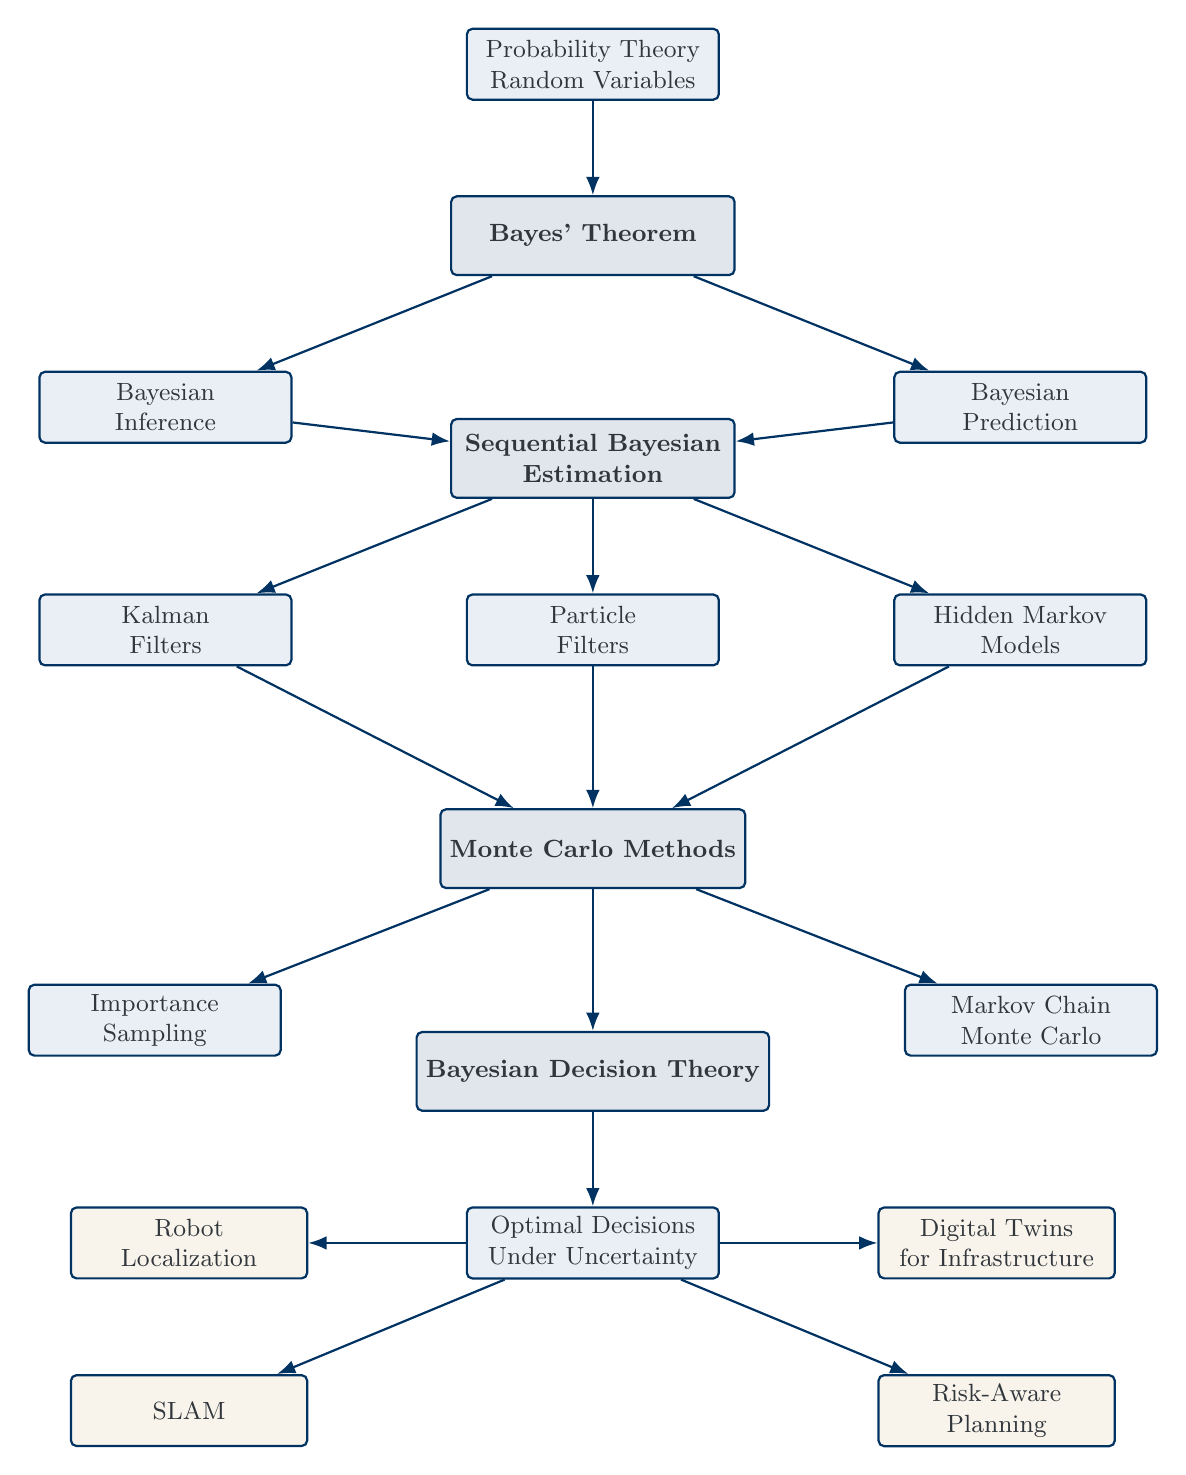
\begin{tikzpicture}[book figure,
node distance=12mm and 20mm,
>=Latex,
concept/.style={
draw,
rounded corners=2pt,
align=center,
minimum width=32mm,
minimum height=9mm,
font=\small,
fill=BookLight
},
core/.style={
draw,
rounded corners=2pt,
align=center,
minimum width=36mm,
minimum height=10mm,
font=\small\bfseries,
fill=BookBlue!12
},
app/.style={
draw,
rounded corners=2pt,
align=center,
minimum width=30mm,
minimum height=9mm,
font=\small,
fill=BookGold!8
},
line/.style={->, draw=BookBlue, line width=0.8pt}
]

%------------------------------------------------
% Foundations
%------------------------------------------------

\node[concept] (prob) {Probability Theory\\Random Variables};

\node[core, below=of prob] (bayes) {Bayes' Theorem};

\node[concept, below left=of bayes] (infer) {Bayesian\\Inference};
\node[concept, below right=of bayes] (predict) {Bayesian\\Prediction};

%------------------------------------------------
% Sequential estimation
%------------------------------------------------

\node[core, below=18mm of bayes] (seq) {Sequential Bayesian\\Estimation};

\node[concept, below left=of seq] (kf) {Kalman\\Filters};
\node[concept, below=of seq] (pf) {Particle\\Filters};
\node[concept, below right=of seq] (hmm) {Hidden Markov\\Models};

%------------------------------------------------
% Monte Carlo
%------------------------------------------------

\node[core, below=18mm of pf] (mc) {Monte Carlo Methods};

\node[concept, below left=of mc] (is) {Importance\\Sampling};
\node[concept, below right=of mc] (mcmc) {Markov Chain\\Monte Carlo};

%------------------------------------------------
% Decision
%------------------------------------------------

\node[core, below=18mm of mc] (decision) {Bayesian Decision Theory};

\node[concept, below=of decision] (opt) {Optimal Decisions\\Under Uncertainty};

%------------------------------------------------
% Applications
%------------------------------------------------

\node[app, left=of opt] (loc) {Robot\\Localization};

\node[app, below left=of opt] (slam) {SLAM};

\node[app, below right=of opt] (plan) {Risk-Aware\\Planning};

\node[app, right=of opt] (dt) {Digital Twins\\for Infrastructure};

%------------------------------------------------
% Arrows
%------------------------------------------------

\draw[line] (prob) -- (bayes);

\draw[line] (bayes) -- (infer);
\draw[line] (bayes) -- (predict);

\draw[line] (infer) -- (seq);
\draw[line] (predict) -- (seq);

\draw[line] (seq) -- (kf);
\draw[line] (seq) -- (pf);
\draw[line] (seq) -- (hmm);

\draw[line] (kf) -- (mc);
\draw[line] (pf) -- (mc);
\draw[line] (hmm) -- (mc);

\draw[line] (mc) -- (is);
\draw[line] (mc) -- (mcmc);

\draw[line] (mc) -- (decision);
\draw[line] (decision) -- (opt);

\draw[line] (opt) -- (loc);
\draw[line] (opt) -- (slam);
\draw[line] (opt) -- (plan);
\draw[line] (opt) -- (dt);

\end{tikzpicture}
\end{document}
